\chapter{Das ELF-Dateiformat}
ELF (\textit{Executable and Linking Format}) ist das Standard-Binärformat von vielen UNIX-ähnlichen Betriebssystemen.
Es wird für ausführbare Dateien und auch für Libraries verwendet.
Es können auch notwendige Informationen für den Debugger in dieses Format gepackt werden.

% TODO: besser embeddet anwendung beschreiben
Das ELF-Format wird auch für Embedded-Anwendungen verwendet.
Das Cross-Kompilierte Programm kann zusammen mit Debug-Informationen in eine ELF-Datei gepackt werden.
Der \textit{gdb} kann dann genutzt werden, um die Applikation auf das Target zu laden.
Im Anschluss kann der \textit{gdb} gleich als Debugger für die Applikation genutzt werden, da alle Notwendigen Informationen in der ELF-Datei vorhanden sind.

In diesem Kapitel wird der grundlegende Aufbau des Formats erklärt.
Zusätzlich wird auf einige Details genauer eingegangen, die für einen Debugger relevant sind.

Einen sehr guten Einstieg bietet auch der Artikel \textit{''Understanding the ELF''}\footnote{\ \ Direkter Link: \ \ \ \ \ \ \ \ \ https://medium.com/@MrJamesFisher/understanding-the-elf-4bd60daac571\\ Archivierter Link: https://web.archive.org/web/20180705122234/https://medium.com/@MrJamesFisher/understanding-the-elf-4bd60daac571} von James Fisher.
In der Spezifikation für das ELF-Format\cite{bib:ELFSpecification} ist der Aufbau des Formats im Detail erklärt.


\section{Nützliche Tools im Umgang mit ELF-Dateien}
\textit{readelf} ist ein nützliches Linux-Tool um Informationen einer ELF-Datei anzeigen zu lassen.
Unter Windows kann diese Software ebenfalls in der Shell verwendet werden, wenn die \textit{''GNU Embedded Toolchain''} installiert wurde.
Im Kapitel \ref{section:installationGDB} wird beschrieben, wie die Toolchain installiert werden kann.
% mingw

\section{Grundlegender Aufbau}
\begin{figure}[htbp]
	\centering
		% 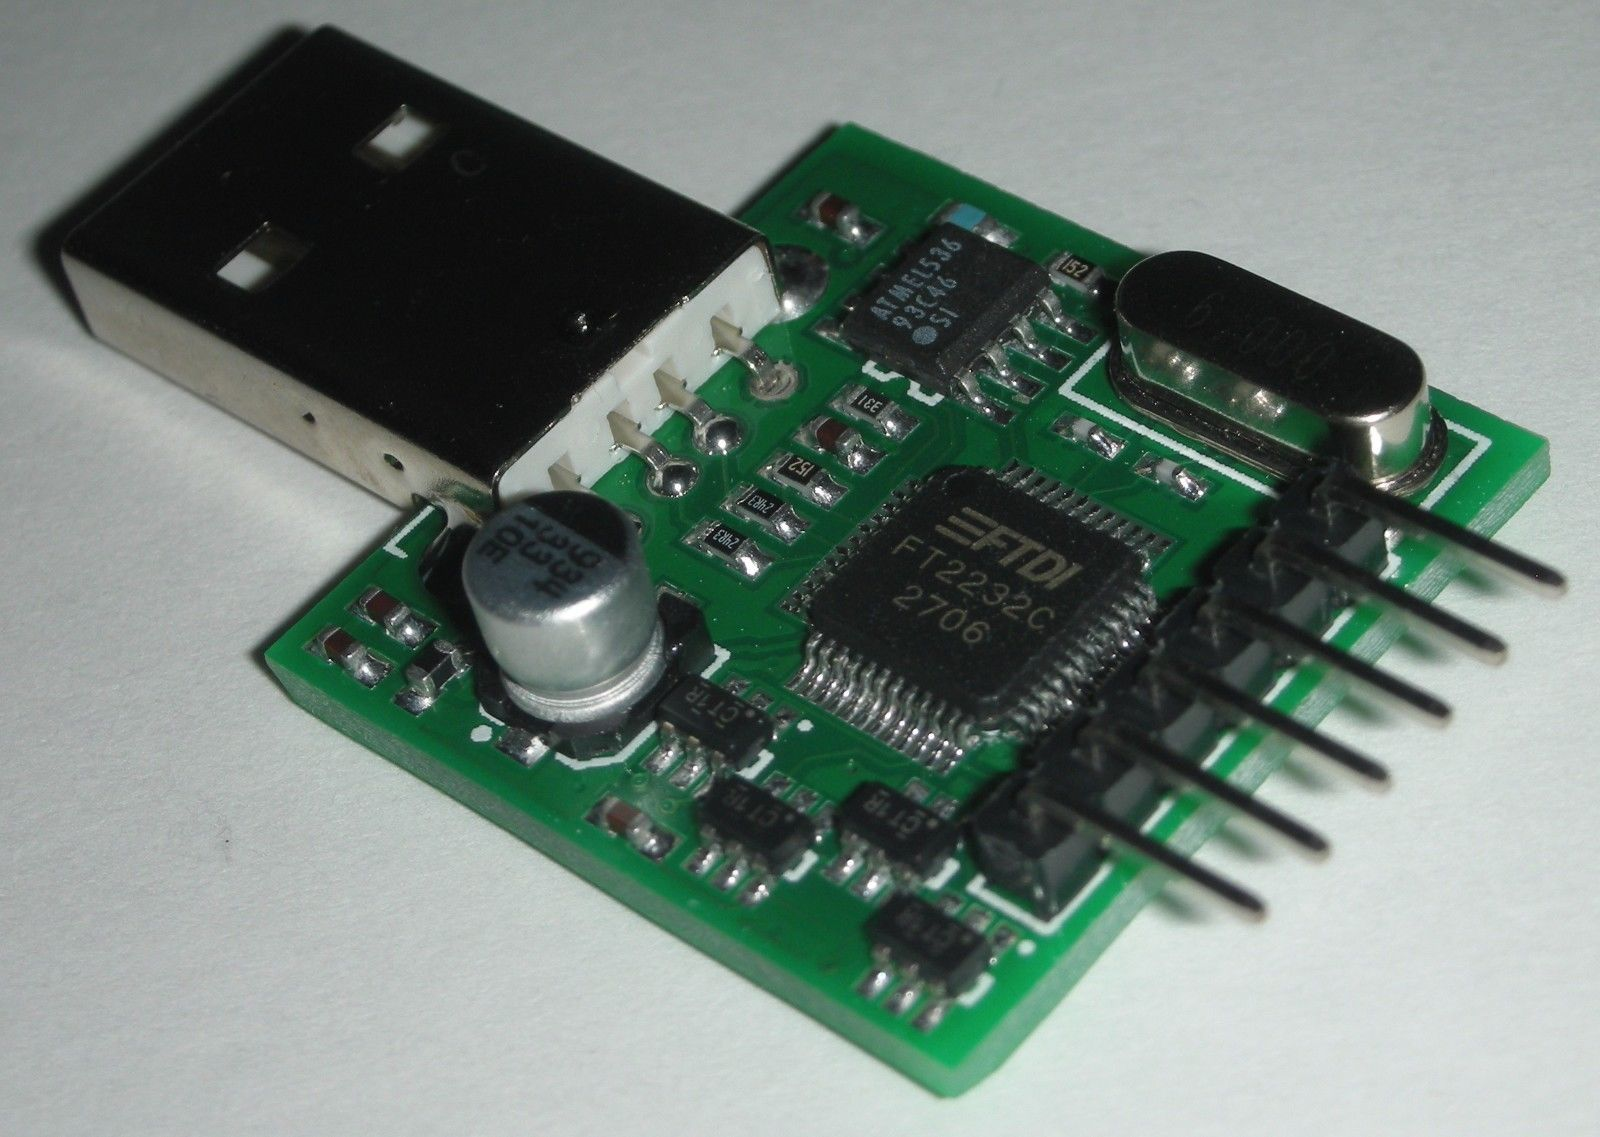
\includegraphics[width=\textwidth,height=\textheight,keepaspectratio]{images/JTAGAdapter.jpg}
		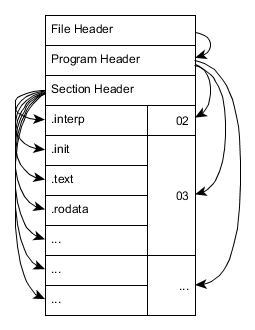
\includegraphics[width=7cm,keepaspectratio]{graphs/elf.png}
	\caption[Der Aufbau von einer ELF Datei]{Der Aufbau von einer ELF Datei\footnotemark}
	\label{fig:ELFStructure}
\end{figure}
\footnotetext{https://slideplayer.com/slide/6444592/}

% Auf Wikipedia\footnote{https://en.wikipedia.org/wiki/Executable\_and\_Linkable\_Format} ist der Aufbau sehr gut beschrieben.


% \begin{figure}[htbp]
% 	\centering
% 		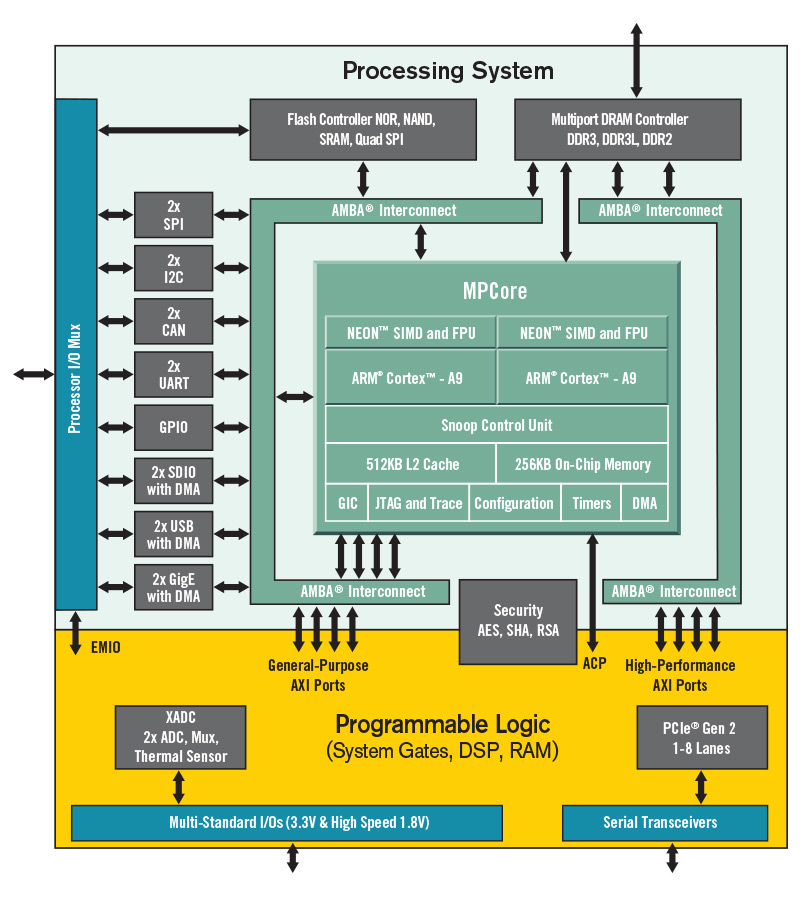
\includegraphics[width=10cm,height=\textheight,keepaspectratio]{images/zynqBlockDiagram.png}
% 	\caption[Block Diagramm Zynq\-7000]{Block Diagramm Zynq\-7000\footnotemark}
% 	\label{fig:BlockDiagrammZynq}
% \end{figure}
% \footnotetext{https://www.xilinx.com/products/silicon-devices/soc/zynq-7000.html}

Der \textit{File Header} beinhaltet Metainformationen über die Datei selbst.
Mit \texttt{''readelf filename -Wh''} lässt sich der \textit{File Header} einer Datei anzeigen.

Der \textit{Program Header} kann mit \texttt{''readelf filename -Wl''} ausgegeben werden.
Darin ist enthalten, welchen Offset die einzelnen Segmente innerhalb der Datei haben.
Zusätzlich ist auch definiert, zu welcher Speicheradresse (im RAM) die Segmente kopiert werden, wenn das Programm gestartet wird und was für Rechte (ausführbar, lesen und schreiben) jedes Speichersegment hat.
Wird, z.B. wegen eines nicht initialisierten Pointers, in einer Speicherstelle im Memory gelesen, die kein \textit{''read flag''} hat, wird ein \textit{Segmentation Fault} ausgelöst.
% TODO: welches segment wird beim gdb geschrieben?
Der \textit{gdb} nutzt Informationen aus diesem Header um zu bestimmen, welche binären Daten mit dem Befehl \texttt{''load''} an welchen Speicherort der Programmcode, die Variablen und die Konstanten kopiert werden sollen.
Ein Segment beinhaltet ein oder mehrere \textit{Sections}.
% TODO: satz sollte klarer sein
% Die Segmente sind beim Ausführen der Datei relevant.

Im \textit{Section Header} sind alle \textit{Sections} beschrieben.
Mit \texttt{''readelf filename -WS''} kann man sehen, dass jede \textit{Section} unter anderem einen Namen, einen Typ, eine Adresse (absolut) und einen Offset (relativ, innerhalb der ELF-Datei) enthält.
Jede \textit{Section} beinhaltet einen anderen Teil des Programms.
Die folgende Liste gibt eine nicht vollständige Übersicht über die einzelnen \textit{Sections}:
\begin{itemize}
	\item \texttt{.text}\ \ \ \ \ \ \ \ \ Der ausführbare Teil des Programms.
	\item \texttt{.data}\ \ \ \ \ \ \ \ \ Enthält die globalen Variablen.
	\item \texttt{.rodata}\ \ \ \ \ Enthält alle Strings.
	\item \texttt{.stab}\ \ \ \ \ \ \ \ \ Enthält die STABS Debuginformationen. Mehr dazu im Kapitel \ref{label:stabs} 
	\item \texttt{.stabstr}\ \ \ Enthält die STABS Debuginformationen. Mehr dazu im Kapitel \ref{label:stabs} 
\end{itemize}
Der Compiler nutzt die \textit{Secitons}, um das Programm in logische Einheiten zu unterteilen.
% Eine \textit{Seciton} ist eine Logische Einheit eines Programms, deren Einteilung besonders für den Compiler Vorteile bringt.


\subsection{Informationen für den Debugger}
Zusätzliche Informationen für den Debugger werden ebenfalls im ELF-Format gespeichert.
Moderne Compiler verwenden hauptsächlich das DWARF-Format und nicht das veraltete STABS-Format.
Trotzdem wird von aktuellen Compilern und auch Debuggern das veraltete STABS-Format immer noch unterstützt.

DWARF ist flexibler und hat einen besseren funktionalen Umfang als das STABS-Format, aber die manuelle Implementation ist aufwändiger.



\section{STABS}
\label{label:stabs}
% TODO: Debugging-Informationen oder Debugginginformationen.
STABS ist ein Datenformat für Debug-Informationen.
Die Informationen sind als Strings in \textit{\textbf{S}ymbol \textbf{TA}ble \textbf{S}trings} gespeichert.
% Obwohl dieses Format veraltet ist, wird dieses Format in dieser Arbeit verwendet, weil es am einfachsten manuell zu implementieren ist.
% Bei moderneren Systemen wurde das STABS-Format durch das neuere DWARF-Format abgelöst.

\subsection{Zielsetzung}
Es soll getestet werden, ob es möglich ist, eine \textit{deep}-Applikation mit dem \textit{gdb} zu debuggen.
Dazu benötigt der \textit{gdb}, neben dem ausführbaren Maschinencode, zusätzliche Debug-Informationen in der Form von STABS oder im DWARF-Format.
In beiden Fällen werden die Informationen im ELF-Format eingebettet.

In dieser Arbeit wird ein Demoprogramm mit STABS implementiert, da STABS-Informationen einfacher manuell zu implementieren sind als DWARF-Informationen.


\subsection{Aufbau des STABS-Format}
Eine einheitliche Dokumentation für STABS gibt es nicht.
Es ist nicht einmal sicher bekannt, wer der ursprüngliche Erfinder dieses Formats ist.
In der Dokumentation von \textit{Sourceware}\footnote{\ \ Direkter Link: \ \ \ \ \ \ \ \ \ https://www.sourceware.org/gdb/onlinedocs/stabs.html\\ Archivierter Link: \ \ \ https://web.archive.org/web/20180717131349/https://www.sourceware.org/gdb/onlinedocs/stabs.html} wird aber Peter Kessler als Erfinder genannt.

Der Aufbau dieses Formats wird in der oben genannten Dokumentation von \textit{Sourceware} und in der Dokumentation der \textit{''University of Utha''}\footnote{\ \ Direkter Link: \ \ \ \ \ \ \ \ \ http://www.math.utah.edu/docs/info/stabs\_toc.html\\ Archivierter Link: \ \ \ https://web.archive.org/web/20180717132825/http://www.math.utah.edu/docs/info/stabs\_toc.html} beschrieben.
Obwohl diese Dokumentationen zum Teil sehr detailliert sind, sind sie nicht lückenlos.
Im Folgenden wird nur auf die Grundlagen eingegangen, die für die Demo-Applikation relevant sind.

STABS-Informationen sind in einzelne Informations-Elemente, sogenannte \textit{directives}, unterteilt.
Jede Direktive ist entweder ein \textit{''.stabs''} (String), ein \textit{''.stabn''} (Integer) oder ein \textit{''.stabd''} (Dot).
Zusätzlich hat jede Direktive einen bestimmten Typ.
Der Typ definiert, was die einzelnen Direktiven genau beschreiben.
Um die Leserlichkeit zu verbessern sind alle Typen in der Datei \textit{''stabs.include''} (Siehe Anhang \ref{anhang:stabs.include}) definiert.
Im Kapitel 12 der Dokumentation der \textit{''University of Utha''} sind die einzelnen Typen genau beschrieben.
% TODO grafische übersicht stabs-stabstring-typ

Die STABS werden mit folgender Syntax im Assembler-Code definiert:\\
\lstset{language=plain}
\begin{lstlisting}
.stabs ''string'',type,other,desc,value
.stabn type,other,desc,value
.stabd type,other,desc
\end{lstlisting}



\subsection{DWARF}
% TODO: DWARF erklären


\section{Demoprogramm mit STABS}
\label{section:demoprogrammSTABS}
% TODO alle files im Anhang
In diesem Kapitel wird beschrieben wie ein Demoprogramm mit STABS-Informationen erstellt werden kann.
Das Demoprogramm soll dann mit dem \textit{gdb} direkt auf den Zynq geladen werden.
Zusätzlich sollen folgende \textit{gdb}-Features getestet werden:\\
\begin{enumerate}
	\item \textbf{Breakpoint}: Das Programm stoppt bei einer gewünschten Zeile im Java-Sourcecode.
	\item \textbf{Sourcecode-Lookup}: Wenn das Programm gestoppt wird, kann die entsprechende Zeile im Java-Sourcecode angezeigt werden.
	\item \textbf{Single-Stepping}: Nur eine Zeile im Java-Sourcecode ausführen und dann pausieren.
	\item \textbf{Variable auslesen}: Eine Java-Variable, z.B. ein Integer, auslesen.
	\item \textbf{Variable manipulieren}: Eine Java-Variable verändern.
	\item \textbf{Prozessor-Register auslesen}: Ein Register der CPU auslesen.
\end{enumerate}


\subsection{Vorgehen}
Um ein Demoprogramm zu erstellen, werden die untenstehenden Schritte durchgeführt.
Alle Schritte werden weiter unten im Detail erklärt.
Das Programm \textit{''loop''}, beziehungsweise \textit{''loopWithSTABS''}, soll für den \textit{gdb}-Test verwendet werden.
\textit{''loopExample''} ist ein Hilfsprogramm, das vom \textit{gdb} automatisch generierte STABS enthält.
Es dient als Vorlage, um die korrekten STABS im Programm \textit{''loop''} hinzufügen zu können.

% Das Demoprogramm 
\begin{enumerate}
	\item \textbf{loop.java}: Demoprogramm als Java-Code Schreiben.
	% deep: java -> maschine
	\item Beispiel-Programm mit automatisch generierten STABS erstellen:
	\begin{enumerate}
		\item \textbf{loopExample.c}: Das Java-Programm manuell in C-Code übersetzen.
		\item \textbf{loopExample.o}: Das Programm mit STABS-Informationen kompilieren.
		\item \textbf{loopExample.Sd}: Das disassemblierte Programm mit STABS in einer leserlichen Form.
		\item \textbf{loopExample.host.c}: Leicht abgeändertes \textit{''loopExample.c''}, um ein ausführbares Programm für den Host-PC zu erhalten.
		\item \textbf{loopExample.host.a}: Ausführbares Programm für den Host-PC.
	\end{enumerate}
	\item Lauffähiges Demoprogramm für den Zynq mit manuell ergänzten STABS erstellen:
	\begin{enumerate}
		\item \textbf{Reset.Java}: Den Sourcecode des Java-Programms in die Reset-Methode des \textit{deep}-Kernel kopieren.
		\item Den modifizierten Kernel mit \textit{deep} übersetzen.
		\item \textbf{loopMachineCode.txt}: Enthält den Maschinen-Code aus der \textit{ClassTreeView} von \textit{deep}.
		\item \textbf{loop.S}: Der aus \textit{''loopMachineCode.txt''} abgeleitete Assembler-Code.
		\item \textbf{loopWithSTABS.S}: Der Assembler-Code inklusive den manuell ergänzten STABS.
		\item \textbf{loopWithSTABS.o}: Kompiliertes Objekt aus dem Assembler-Code.
		\item \textbf{loopWithSTABS}: Gelinktes Objekt aus dem kompilierten Objekt.
		\item \textbf{loopWithSTABS.Sd}: Das disassemblierte Programm mit STABS in einer leserlichen Form.
	\end{enumerate}
\end{enumerate}



\subsection{Java Demoprogramm}
Das untenstehende Programm ist das Testprogramm (loop.java), dass von \textit{deep} in Maschinen-Code übersetzt werden soll und anschliessend manuell mit STABS ergänzt werden soll.

\textbf{loop.java:}
\lstset{language=java}
\begin{lstlisting}
static void reset() {



	US.PUTGPR(SP, stackBase + stackSize - 4);	// set stack pointer
	
	int x00 = 0;
	int x01 = 1;
	int x02 = 2;
	
	x00++;
	x01++;
	x02++;
	
	int x100 = 100;
	for(int i=0; i<10; i++){
		x100 += 10;
   }
		
	x100++;
	x100++;
	x100++;
	x100++;
	x100++;

	US.ASM("b -8"); // stop here
}
\end{lstlisting}

In diesem Beispiel wird die \texttt{reset()}-Methode genutzt, da sie bei \textit{deep} als erstes beim Booten ausgeführt wird.
\texttt{''US.PUTGPR''} in Zeile 5 ist natürlich keine Java-Methode.
Da Low-Level-Operationen, wie die Initialisierung des Stackpointers, mit Java normalerweise nicht möglich sind, wird hier die entsprechende \textit{deep}-Instruktion verwendet.


\subsection{Beispiel-Programm ''loopExample''}
Der Code in \textit{''loopExample.c''} im Anhang \ref{anhang:loopExample.c} ist fast identisch mit dem Code des Java Demoprogramms.
Es wurden nur einige Änderungen vorgenommen, damit der Code als C-Programm kompiliert werden kann.
\texttt{c\_entry()} ist der Eintrittspunkt des Programms und erfüllt im embedded Bereich eine ähnliche Aufgabe wie die  \texttt{main()}-Methode in einem generischen C-Programm.

Mit dem PowerShell-Script \textit{''make\_loopExample.ps1''} im Anhang \ref{anhang:make_loopExample.ps1} kann das C-Programm kompiliert werden.
Es erzeugt das Object-File \textit{''loopExample.o''} inklusive Debuginformationen im STABS-Format.
Das disassemblierte Object-File wird als \textit{''loopExample.Sd''} gespeichert.
Im disassemblierten Object-File sind alle STABS-Informationen und auch der ausführbare Code als Assembler enthalten.
Der Assembler-Code und auch die STABS-Informationen können direkt \textit{''human readable''} gelesen werden, aber sie können nicht direkt in einem kompilierbaren Programm verwendet werden, da die Syntax nicht übereinstimmt.

Beispiel mit disassemblierter Syntax:
\lstset{language=plain}
\begin{lstlisting}
...
2      LSYM   0      0      00000000 44     int:t(0,1)=r(0,1);-2147483648;2147483647;
...
00000000 <c_entry>:
   0:	e92d0810 	push	{r4, fp}
\end{lstlisting}


Kompilierbare Assembler Syntax:
\lstset{language=plain}
\begin{lstlisting}
...
.stabs "int:t(0,1)=r(0,1);-2147483648;2147483647;",N_LSYM,0,0,0
...
c_entry:
push {r4, fp}
\end{lstlisting}


\subsection{Analyse der disassemblierten STABS}
\FloatBarrier

Die untenstehenden Direktiven sind ein Auszug aus der Datei \textit{''loopExample.Sd''} im Anhang \ref{anhang:loopExample.Sd}.
Die Tabelle \ref{t-DisassemblierteSTABdirektive} beschreibt die Direktive 0 im Detail.
\lstset{language=plain}
\begin{lstlisting}
Symnum n_type n_othr n_desc n_value  n_strx String
...
0      SO     0      2      00000000 15     loopExample.c
1      OPT    0      0      00000000 29     gcc2_compiled.
2      LSYM   0      0      00000000 44     int:t(0,1)=r(0,1);-2147483648;2147483647;
...
51     GSYM   0      0      00000000 1919   global:G(0,1)
52     FUN    0      0      00000000 1933   c_entry:F(0,1)
53     SLINE  0      4      00000000 0 
54     SLINE  0      5      0000000c 0     
...
72     LSYM   0      0      fffffff0 1948   x00:(0,1)
73     LSYM   0      0      ffffffec 1958   x01:(0,1)
74     LSYM   0      0      ffffffe8 1968   x02:(0,1)
75     RSYM   0      0      00000004 1978   s:r(0,1)
76     LSYM   0      0      ffffffe4 1987   float0:(0,14)
77     LSYM   0      0      fffffff8 2001   int0:(0,1)
78     LBRAC  0      0      00000000 0      
79     LSYM   0      0      fffffff4 2012   i:(0,1)
80     LBRAC  0      0      00000060 0      
81     RBRAC  0      0      00000090 0      
82     RBRAC  0      0      000000c4 0      
83     SO     0      0      000000c4 0 
\end{lstlisting}

\begin{table}[H]
\caption{Disassemblierte STAB-Direktive}
\label{t-DisassemblierteSTABdirektive}
\begin{tabular}{|l|l|l|}
 \hline
\textit{Symnum}   & 0             & Eindeutige Identifikation der STAB-Direktive \\ \hline
\textit{n\_type}  & S0            & \begin{tabular}[c]{@{}l@{}}Typ der STAB-Direktive. Die SO-Direktive beschreibt das Source-File\\
									 welches die \texttt{''main()''}-Methode enthält. \end{tabular}                                       \\ \hline
\textit{n\_othr}  & 0             & Das \textit{other}-Feld wird normalerweise nicht genutzt und auf ''0'' gesetzt.                                         \\ \hline
\textit{n\_desc}  & 2             & \textit{''the starting text address of the compilation.''}\footnote{http://www.math.utah.edu/docs/info/stabs\_12.html\#SEC73}                                        \\ \hline
\textit{n\_value} & 00000000      & Dieser Integer wird hauptsächlich für \textit{.stabn}-Direktive genutzt.                                         \\ \hline
\textit{n\_strx}  & 15            & Start des Strings der nächste Direktive                                         \\ \hline
\textit{String}   & loopExample.c & \begin{tabular}[c]{@{}l@{}}Der String, der die eigentliche Information enthält. In diesem Fall\\ 
									ist es das Source-File mit der \texttt{''main()''}-Methode.\end{tabular}            \\  \hline                           
\end{tabular}
\end{table}
% TODO: the starting text address of the compilation

Die Direktiven 2 bis 50 beschreiben alle Variablentypen.
Für das Testprogramm \textit{''loop''} können diese einfach kopiert werden.

Die GSYM-Direktive deklariert eine globale Variable.
Direktive Nummer 52, vom Typ FUN, definiert eine Methode.

Die Direktiven 53 bis 71 sind vom Typ SLINE.
Sie werden für die \textit{Sourcecode-Lookup}-Funktion verwendet.
\textit{n\_desc} beschreibt die Zeile im Sourcecode und \textit{n\_value} die entsprechende Adresse im Maschinencode.
Es fällt auf, dass die Sourcecode-Adresse von der Direktive 53 auf 54 nur um eine Zeile steigt, die Maschinencode-Adresse aber von 00000000 auf 0000000c.
Im Gegensatz zur Zeilennummer, wird die Adresse im Maschinencode im Hexadezimalen System angegeben.
Da es sich um 32-Bit lange Maschinen-Instruktionen (also 4 Byte) handelt, steigt die Adresse um 4 nach jeder Instruktion.
Es werden also drei Maschinen-Instruktionen ausgeführt, bevor die erste Zeile in der Methode \texttt{''c\_entry()''} ausgeführt wird.
Im disassemblierten Maschinencode sieht man folgende Instruktionen:
\lstset{language=plain}
\begin{lstlisting}
   0:	e92d0810 	push	{r4, fp}
   4:	e28db004 	add	fp, sp, #4
   8:	e24dd018 	sub	sp, sp, #24
   c:	e3a03000 	mov	r3, #0
  10:	e50b3010 	str	r3, [fp, #-16]
\end{lstlisting}

Wie es aussieht, wird der Stackpointer mit den ersten drei Instruktionen initialisiert, bevor die erste Zeile, oder genauer gesagt Zeile 5, in \textit{''looopExample.c''}, ausgeführt wird.

Die LSYM-Direktiven ab Nr. 72 definieren Variablen, welche auf dem Stack gespeichert sind.
Mit \textit{n\_value} wird die Adresse der Variable im Speicher definiert.
Der \textit{String} definiert den Variablennamen ''x00'' und den Typ ''(0,1)''.
Der Typ ''(0,1)'' wurde mit der Direktive 2 als Integer definiert.

Die Direktive 75 definiert eine Variable, die nicht auf dem Stack gespeichert wird.
Dieser Typ wird verwendet, wenn die Variable nur in einem Prozessor-Register gespeichert und nicht auf dem Stack abgelegt wird.
Der \textit{gcc} speichert grundsätzlich alle Variablen direkt auf dem Stack wenn sie erzeugt oder verändert werden und lädt sie jedesmal neu vom Stack, wenn sie wieder gelesen werden.
Wird beim Kompilieren eine Code-Optimierung verwendet, kann dieses Verhalten ändern.
Mit der Zeile \texttt{{''register int s=1;''}} im C-Code wird der Compiler gezwungen, die Variable in den Registern zu behalten und nicht auf dem Stack abzulegen.
Aus diesem Grund wird für die Variable \textit{''s''} eine Direktive des Typs RSYM verwendet, die nur den Namen der Variable und die Registernummer beschreibt, in der die Variable gespeichert wird.

Mit STABS können auch lexikalische Blöcke abgegrenzt werden, ähnlich wie mit geschwungenen Klammern ({}) in C-Code.
Zusätzlich wird so auch die Lebensdauer von Variablen begrenzt.
Die Direktiven 78 und 80 (LBRAC) markieren einen Start und die Direktiven 81 und 82 (RBRAC) markieren jeweils das Ende eines solchen Blocks.


\subsection{Assemblerprogramm mit \textit{deep} erzeugen}
Um das Java-Programm möglichst einfach mit \textit{deep} übersetzen zu können, wird die \texttt{''reset()''}-Methode des Objekts \textit{''Reset.java''} aus dem Package \textit{''zynq7000''} überschrieben.
% TODO satzbau:
Diese Methode wird beim Starten einer \textit{deep}-Applikation immer als erstes ausgeführt und ist somit mit einem Debugger gleich ab der ersten Instruktion der Applikation kontrollierbar.

Die untenstehenden Zeilen entsprechen den Zeilen 39-42 von \textit{''Reset.java} aus dem Anhang \ref{anhang:reset.java}.
In diesen Zeilen wird die Position des Stacks ausgerechnet und im Stackpointer gespeichert:
\lstset{language=java}
\begin{lstlisting}
int stackOffset = US.GET4(sysTabBaseAddr + stStackOffset);
int stackBase = US.GET4(sysTabBaseAddr + stackOffset + 4);
int stackSize = US.GET4(sysTabBaseAddr + stackOffset + 8);
US.PUTGPR(SP, stackBase + stackSize - 4);	// set stack pointer
\end{lstlisting}

Wird ein Dummy-Programm mit dem \textit{deep}-Compiler und dem modifiziertem Kernel kompiliert, dann wird auch der Kernel kompiliert.
Mit der \textit{ClassTreeView} (siehe Abbildung \ref{fig:MaschineCode.ClassTreeView.Deep}) von \textit{deep} kann der Assemblercode der \texttt{''reset()''}-Methode kopiert werden, welcher im Anhang \ref{anhang:loopMachineCode.txt} angehängt ist.

\begin{figure}[htbp]
	\centering
		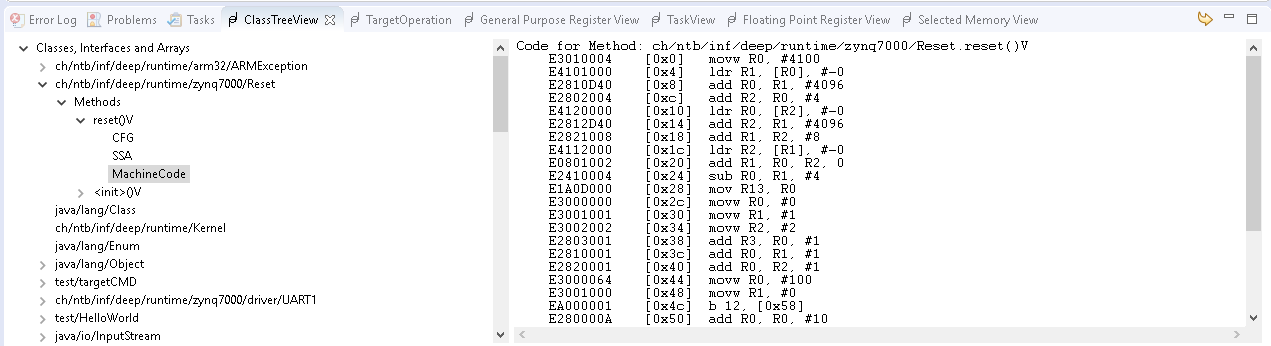
\includegraphics[width=\textwidth,height=\textheight,keepaspectratio]{images/MaschineCode_ClassTreeView_Deep.PNG}
	\caption[]{ClassTreeView mit Maschinencode der Reset-Methode in \textit{deep}}
	\label{fig:MaschineCode.ClassTreeView.Deep}
\end{figure}


\FloatBarrier

loop.S:
\lstset{language={[x86masm]Assembler}}
\begin{lstlisting}
.global _start

.org 0x000000
.text
Ltext0:

_start:
_reset:
c_entry:
movw R13, #1024

movw R0, #0
movw R1, #10
movw R2, #20
add R3, R0, #1
add R0, R1, #1
add R0, R2, #1
movw R0, #100
movw R1, #0
b CHECK_LOOP_EXIT	
START_LOOP_BODY:
add R0, R0, #10
add R1, R1, #1
CHECK_LOOP_EXIT:
cmp R1, #10
blt START_LOOP_BODY
add R1, R0, #1
add R0, R1, #1
add R1, R0, #1
add R0, R1, #1
add R1, R0, #1
END:
b END
\end{lstlisting}

% TODO aufgeräumt gut?
\textit{''loop.S''} im Anhang \ref{anhang:loop.S} enthält den ''aufgeräumten'' Assemblercode.
Der Code wurde mit zusätzlichen Assembler-Direktiven ergänzt.
\texttt{''c\_entry''} beschreibt den Start des Programms.
\texttt{''START\_LOOP\_BODY''} und \texttt{''CHECK\_LOOP\_EXIT''} sind Punkte, welche für die \textit{For-Loop} benötigt werden.

In Zeile 10 wird der Stackpointer direkt mit einer Konstante gesetzt und nicht mehr mit \textit{deep}-Konstanten ausgerechnet.
Zusätzlich kann so auch sichergestellt werden, dass der Stack in einem erlaubten Speicherbereich im OCM angelegt wird.

Die beiden Branch-Instruktionen wurden mit der korrekten Syntax ersetzt.
Als Ziel für diese Instruktionen wurden die beiden Assembler-Direktiven \texttt{''START\_LOOP\_BODY''} und \texttt{''CHECK\_LOOP\_EXIT''} verwendet.


\subsection{STABS in das Assemblerprogramm einfügen}
Um das Assemblerprogramm mit STABS zu ergänzen wurden drei verschiedene Quellen genutzt.
Das fertige Assemblerprogramm mit STABS ist im Anhang \ref{anhang:loopWithAssembler.S} angehängt.

Die NTB-Wiki-Dokumentation\footnote{https://wiki.ntb.ch/infoportal/software/gdb/start?s[]=stabs} wurde als Ausgangslage genutzt.
Die Datei \textit{''stabs.include''} (siehe Anhang \ref{anhang:stabs.include}) konnte direkt genutzt werden.
Die Definition des Sourcecods (N\_SO) und die Definitionen der Zeilennummern (N\_SLINE) konnten ebenfalls übernommen werden.

Da die Definitionen der Variablen-Typen in der NTB-Wiki-Dokumentation nicht vollständig waren, konnten sie leider nicht verwendet werden.
Alle Variablendefinitionen, Zeilen 6-75, wurden aus dem disassemblierten Demoprogramm kopiert.
Bei der For-Loop ist die Definition der Sourcecode-Zeile ebenfalls etwas speziell, da sie auch bei der Überprüfung der Exit-Condition stimmen muss.
Die genaue Implementation für die For-Loop wurde ebenfalls aus dem disassemblierten Demoprogramm übernommen.

Sofern noch genügend Register frei sind, scheint der \textit{deep}-Compiler die Variablen nicht auf dem Stack zu sichern.
Zusätzlich werden die Variablen in den Registern überschrieben, wenn diese im späteren Programmverlauf nicht mehr verwendet werden.
Eine Register-Variable wird mit einer Direktive des Typs 'N\_RSYM' definiert, die auf ein bestimmtes Register zeigt.
So werden beispielsweise die Register-Variablen \texttt{x00}, \texttt{x01} und \texttt{x02} in den Zeilen 84, 89 und 94 definiert.

\lstset{language={[x86masm]Assembler},
  firstnumber=84,
  numberfirstline=true}
\begin{lstlisting}
.stabs "x00:r(0,1)",N_RSYM,0,4,0
\end{lstlisting}

\lstset{language={[x86masm]Assembler},
  firstnumber=89,
  numberfirstline=true}
\begin{lstlisting}
.stabs "x01:r(0,1)",N_RSYM,0,4,1
\end{lstlisting}

\lstset{language={[x86masm]Assembler},
  firstnumber=94,
  numberfirstline=true}
\begin{lstlisting}
.stabs "x02:r(0,1)",N_RSYM,0,4,2
\end{lstlisting}
\lstset{firstnumber=1}


Auf der Sourcecode-Zeile 11 wird die Variable \texttt{x00} um 1 inkrementiert.
Im Assemblercode sieht man, dass die Variable neu im Register 3 abgespeichert wird.
Aus diesem Grund muss die Register-Variable neu definiert werden.

\lstset{language={[x86masm]Assembler},
  firstnumber=98,
  numberfirstline=true}
\begin{lstlisting}
# x00++;
.stabn N_SLINE, 0, 11, LM11
.stabn N_LBRAC, 0, 0, LM11
.stabs "x00:r(0,1)",N_RSYM,0,4,3
LM11:
add R3, R0, #1
\end{lstlisting}
\lstset{firstnumber=1}



\subsection{Demoprogramm mit STABS kompilieren}
Das Assemblerprogramm enthält nun alle notwendigen Informationen für den Maschinencode in Form von Assemblerinstruktionen.
Die STABS ergänzen das Programm mit allen Informationen, welche der Debugger benötigt.

Mit dem Script \textit{''make\_loop.ps1''} im Ahang \ref{anhang:make_loop.ps1} kann das Programm assembliert werden.
Die ELF-Datei \textit{''loopWithSTABS''} kann dann mit dem \textit{gdb} geladen werden.


